
\documentclass{report}

\usepackage{amsthm}
\usepackage[top=2.5cm, left=2.5cm, right=2.5cm, bottom=2.5cm]{geometry}
\usepackage{tikz-cd}

\theoremstyle{plain}
\newtheorem{thm}{Theorem}[section]
\newtheorem{lem}[thm]{Lemma}
\newtheorem{prop}[thm]{Proposition}
\newtheorem*{cor}{Corollary}

\theoremstyle{definition}
\newtheorem{defn}{Definition}[section]
\newtheorem{conj}{Conjecture}[section]
\newtheorem{exmp}{Example}[section]

\theoremstyle{remark}
\newtheorem*{rem}{Remark}
\newtheorem*{note}{Note}


\begin{document}
%\begingroup
\title{Categories and music}
\author{Alice Rixte}
\date{\today}
\maketitle %\endgroup


\chapter{Introduction}
\section{Presentation of PK-nets}
\begin{defn}\textbf{Set} is the category where objects are the sets and morphisms are functions between sets.\end{defn}


\begin{figure}[h]
    \centering
    \label{PK-net definition}
    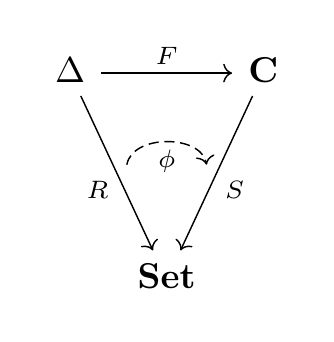
\begin{tikzpicture}[baseline= (a).base]
        \node[scale=1.3] (a) at (0,0){
            \begin{tikzcd}[column sep=tiny]
                \Delta \ar[ddr, "R"',""{name=R,right}] \ar[rr,"F"]	& & \textbf{C} \ar[ddl,"S",""{name=S,left}] \\
                & \ar[dashed,bend left=80,from=R, to=S, "\phi"']& \\
                & \bf Set &
            \end{tikzcd}
        };
    \end{tikzpicture}
\end{figure}



\begin{defn} The category of elements $el(F)$ of a functor $F : \mathcal{C}\rightarrow \textbf{Set}$ is defined as follows :
    \begin{itemize}
        \item its objects are the pairs $(c,x)$ where $c$ is an object of $\mathcal{C}$ and $x\in F(c)$
        \item its morphisms $(c,x)\rightarrow (c',x')$ are morphisms $u : c\rightarrow c'$ such that $F(u)(x) = x'$
    \end{itemize}

  

\end{defn}

\paragraph{}
Now, what is the category of elements of the PLR-group action over \textbf{Set}? Let $S$ be the functor from the category PLR to the category \textbf{Set} such that $S$ associates to the only object of PLR a set $X$ of cardinality 24 and such that $S$ is a PLR-group action on $X$.

$el(S)$ is then a category with $24$ objects. One can use it as a $\Delta$ category in a PK-net. The transformation $\phi$ gives us the musical interpretation, of each transformation between triads.

=> How to add more structure to eliminate arrow? Maybe take two generators





\chapter{Conclusion}
\end{document}